\section{Búsqueda}
La función \verb!query! nos ayuda a determinar si es que los datos se encuentran dentro de un espacio 3D. Es una búsqueda por aproximación.

La búsqueda es eficiente porque se limita al octante en específico en donde se encuentra la esfera a ser localizada.

\begin{lstlisting}[caption=Consulta Octree: \textit{Point Region}]
  query(range, found) {
    if (!found) {
      found = [];
    }
    //no se intercepta con los limites del cuadrante
    if (!range.intersects(this.cubo)) {
      return found;
    }
    //Ciclo por cada punto del ocdtree
    for (let p of this.points) {
      //Verificamos si esta dentro del rango
      if (range.contains(p)) {
        //1 1 1 blanco / Cambia este color
        p.material.color.set(new THREE.Color(0, 0, 0));
        //Lo insertamos en el vector found
        found.push(p);
        //count++;
      }
    }
    //Si ha sido dividido
    if (this.divided) {
      //Llamamos recursivamente a cada hijo
      this.northwestf.query(range, found);
      this.northeastf.query(range, found);
      this.southwestf.query(range, found);
      this.southeastf.query(range, found);
      this.northwestb.query(range, found);
      this.northeastb.query(range, found);
      this.southwestb.query(range, found);
      this.southeastb.query(range, found);
    }
    return found;
  }
\end{lstlisting}

A continuación se muestran algunos ejemplos:
\begin{itemize}
    \item Consulta de esferas sobre una región. Ver figura \ref{fig:search01}.
    \begin{figure}[H]
      \centering
      \fbox{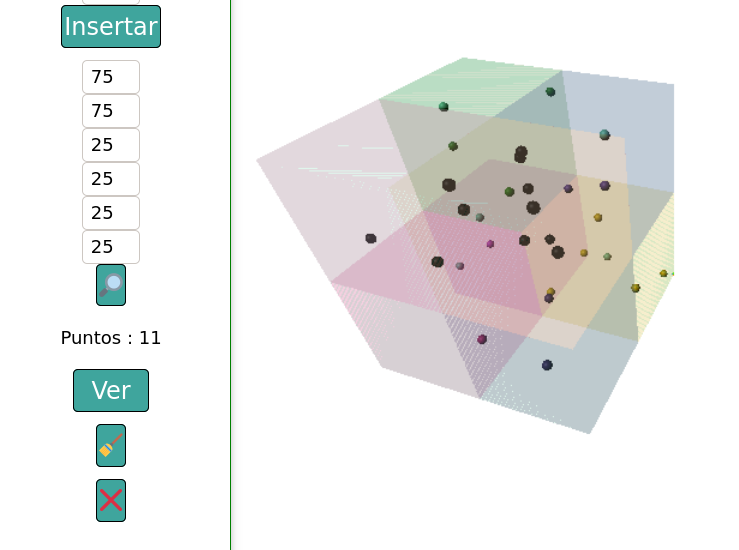
\includegraphics[width=0.55\textwidth]{search01}}
      \caption{Sombreado de las esferas (puntos) en consulta}
      \label{fig:search01}
    \end{figure}
    \item Volumen captado por la consulta cúbica.
    \begin{figure}[H]
      \centering
      \fbox{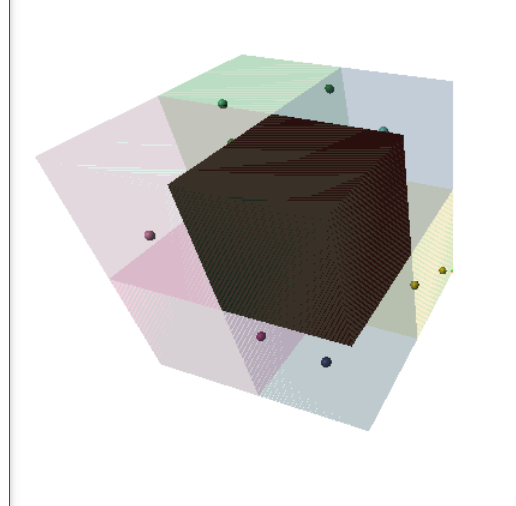
\includegraphics[width=0.55\textwidth]{search02}}
      \caption{Cubic query}
      \label{fig:search02}
    \end{figure}
\end{itemize}



\iffalse
% ---- Para poner dos imágenes (una a lado de otra) ----
Como se muestra en la figuras \ref{fig:act-1_a} y \ref{fig:act-1_b}.
\begin{figure}[H]
\centering
\begin{minipage}{0.75\textwidth}
  \centering
  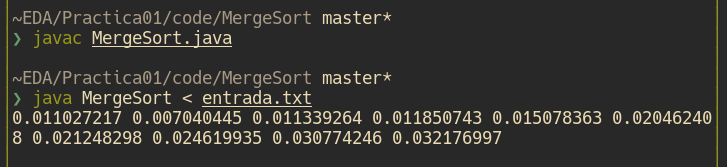
\includegraphics[width=0.8\textwidth]{ejecucion-java}
  \caption{blablablabalbalabla.}
  \label{fig:act-1_a}
\end{minipage}\hfill
\begin{minipage}{0.75\textwidth}
  \centering
  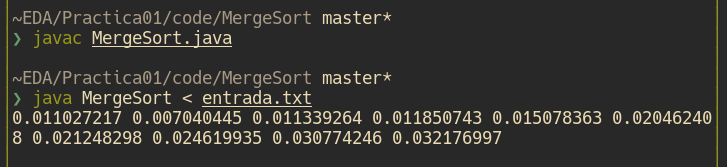
\includegraphics[width=0.8\textwidth]{ejecucion-java}
  \caption{blablablslablala}
  \label{fig:act-1_b}
\end{minipage}
\end{figure}
% ---- Para colocar una imagen ----
Como se muestra en la figura \ref{fig:act-3}
\begin{figure}[H]
  \centering
  \includegraphics[width=0.8\textwidth]{act-3}
  \caption{Tabla de subneteo para la red 192.168.100.0.}
  \label{fig:act-3}
\end{figure}
\fi